\documentclass[10pt,twocolumn,letterpaper]{article}

\usepackage{cvpr}
\usepackage{times}
\usepackage{epsfig}
\usepackage{graphicx}
\usepackage{amsmath}
\usepackage{amssymb}

% SIAM Shared Information Template
% This is information that is shared between the main document and any
% supplement. If no supplement is required, then this information can
% be included directly in the main document.


% Packages and macros go here
\usepackage{lipsum}
\usepackage{amssymb}
\usepackage{amsfonts}
\usepackage{amsopn}
\usepackage{mathtools}
\usepackage{graphicx}
\usepackage{epstopdf}
\usepackage{algorithmic}
\usepackage{tikz}
% \usepackage{pgfplots}
\usetikzlibrary{shapes.arrows, patterns, calc}
\usepackage{tikz-3dplot}
\usepackage{bbm}
\usepackage{bm}
\ifpdf
  \DeclareGraphicsExtensions{.eps,.pdf,.png,.jpg}
\else
  \DeclareGraphicsExtensions{.eps}
\fi
% \usepackage{todonotes}

\definecolor{lightblue}{HTML}{a1b4c7}
\definecolor{orange}{HTML}{ea8810}
\definecolor{silver}{HTML}{b0aba8}
\definecolor{rust}{HTML}{b8420f}
\definecolor{seagreen}{HTML}{23553c}

\colorlet{darklightblue}{lightblue!85!black}
\colorlet{darkorange}{orange!85!black}
\colorlet{lightsilver}{silver!15!white}
\colorlet{darksilver}{silver!85!black}
\colorlet{darkrust}{rust!85!black}
\colorlet{darkseagreen}{seagreen!85!black}

\definecolor{ice}{HTML}{48dbfb}
\definecolor{ore}{HTML}{2c3e50}
\definecolor{rubblelight}{HTML}{f4f4f4}
\definecolor{rubbledark}{HTML}{9f9f9f}

\definecolor{factory1}{HTML}{5aa8ec}
\definecolor{lichen1}{HTML}{90c2ed}
\definecolor{robot1}{HTML}{228be6}

\definecolor{factory2}{HTML}{f46f6f}
\definecolor{lichen2}{HTML}{f2a8a8}
\definecolor{robot2}{HTML}{f03e3e}

% Names of standard objects
\newcommand*{\Reals}{\mathbb{R}}
\newcommand*{\Naturals}{\mathbb{N}}

\newcommand*{\defeq}{\coloneqq}
\newcommand*{\BigO}{\mathcal{O}}
\newcommand*{\N}{\mathcal{N}}
\newcommand*{\SpSet}{\mathcal{S}}
\newcommand*{\GP}{\mathcal{GP}}
\newcommand*{\Loss}{\mathcal{L}}
\newcommand*{\Order}{\mathcal{I}}
\newcommand*{\Reverse}{\updownarrow}
\newcommand*{\I}{I}
\newcommand*{\J}{J}
\newcommand*{\V}{V}

\renewcommand*{\vec}[1]{\bm{#1}}
\newcommand*{\Id}{\text{Id}}

% Names of variables
% covariance matrix
\newcommand*{\CM}{\Theta}
\newcommand*{\mean}{\mu}
\newcommand*{\var}{\sigma^2}
\newcommand*{\std}{\sigma}
% kernel function
\newcommand*{\K}{K}
\newcommand*{\Train}{\text{Tr}}
\newcommand*{\Pred}{\text{Pr}}

% Names of operators
\DeclarePairedDelimiter{\norm}{\lVert}{\rVert}
\DeclarePairedDelimiter{\card}{\lvert}{\rvert}
\DeclarePairedDelimiter{\ceil}{\lceil}{\rceil}
\DeclareMathOperator{\diag}{diag}
\let\trace\relax
\DeclareMathOperator{\trace}{trace}
\DeclareMathOperator{\logdet}{logdet}
\DeclareMathOperator{\chol}{chol}
\DeclareMathOperator{\FRO}{FRO}

\DeclareMathOperator*{\argmin}{argmin}
\DeclareMathOperator*{\argmax}{argmax}

\DeclarePairedDelimiterX{\infdivx}[2]{(}{)}{%
  #1\;\delimsize\|\;#2%
}
\newcommand*{\KL}{\mathbb{D}_{\operatorname{KL}}\infdivx}
\DeclareMathOperator{\p}{\pi}
\DeclareMathOperator{\E}{\mathbb{E}}
\DeclareMathOperator{\Var}{\mathbb{V}ar}
\DeclareMathOperator{\Cov}{\mathbb{C}ov}
\DeclareMathOperator{\Corr}{\mathbb{C}orr}
\DeclareMathOperator{\entropy}{\mathbb{H}}
\DeclareMathOperator{\MI}{\mathbb{I}}
\DeclareMathOperator{\Prob}{\mathbb{P}}
\DeclareMathOperator{\Ind}{\mathbbm{1}}
\DeclareMathOperator{\cw}{\mathsf{cw}}
\DeclareMathOperator{\Uniform}{\text{Unif}}

%%% Local Variables:
%%% mode:latex
%%% TeX-master: "experimental_design_linalg"
%%% End:


% Include other packages here, before hyperref.

% If you comment hyperref and then uncomment it, you should delete
% egpaper.aux before re-running latex.  (Or just hit 'q' on the first latex
% run, let it finish, and you should be clear).
\usepackage[
  pagebackref=true,
  breaklinks=true,
  % letterpaper=true,
  colorlinks,
  bookmarks=false
]{hyperref}

\cvprfinalcopy % *** Uncomment this line for the final submission

\def\cvprPaperID{****} % *** Enter the CVPR Paper ID here
\def\httilde{\mbox{\tt\raisebox{-.5ex}{\symbol{126}}}}

% Pages are numbered in submission mode, and unnumbered in camera-ready
\ifcvprfinal\pagestyle{empty}\fi
\begin{document}

%%%%%%%%% TITLE
\title{CS 7643 Project Report: Behavior cloning for Lux AI Season 2}

\author{
  Stephen Huan\thanks{%
    Georgia Institute of Technology, Atlanta, GA%
  }\\
  % {\tt\small shuan@gatech.edu}
  % For a paper whose authors are all at the same institution,
  % omit the following lines up until the closing ``}''.
  % Additional authors and addresses can be added with ``\and'',
  % just like the second author.
  % To save space, use either the email address or home page, not both
  \and
  Daniel Lu\footnotemark[1]\\
  \and
  Vedaant Shah\footnotemark[1]\\
  \and
  Jerry Xiong\footnotemark[1]
}

\maketitle
%\thispagestyle{empty}

%%%%%%%%% ABSTRACT
% \begin{abstract}
%   \textcolor{red}{TODO}
% \end{abstract}

%%%%%%%%% BODY TEXT
\section{Introduction}\label{sec:intro}

% (5 points) What did you try to do? What problem did you try to
% solve? Articulate your objectives using absolutely no jargon.
The Lux AI challenge is an AI programming competition in which
two teams of robots face off in a resource-gathering simulation.
Submissions range from heuristic-based algorithms to machine learning
approaches, competing on a continually updating, global leaderboard.
In this project, we experiment with a deep learning approach
for imitating the behavior of strong-performing agents in Lux
AI season 2, which ran on Kaggle from January to April 2023.
The project repository can be found at
\href{https://github.com/jxiong21029/LuxS2}{this link}.

\subsection{Problem description}
\label{subsec:problem}

The competition environment is a two-dimensional grid, where each
agent controls a teams of factories and robots (\autoref{fig:map}).
Robots collect resources such as ice and ore from set locations on
the map, return them to the factories to refine them into water and
metal, and use these resources to build and sustain additional robots.
The game has three phases: a bidding phase, in which agents bid starting
resources to determine the factory placement order; a placement phase,
where agents take turns selecting initial factory locations; and finally,
the main phase of the game, where robots are built and controlled.
The final objective is to maximize the growth of a resource
called lichen using water collected throughout the main phase.

\subsection{Motivation}
\label{subsec:motivation}

A number of competitors utilize heuristic-based agents.
These approaches rely on significant understanding of
the environment dynamics, as well as human intuition.
For example, agents might rely on path-finding algorithms,
or heuristics to delegate robot responsibilities.
Such approaches can scale poorly in terms of
computational cost as the number of agents increases.
In addition, modifying such an approach requires
manually changing the code of the underlying program.

In this project, we examine an deep learning approach
based on imitating the behavior of other agents.
This approach can not only leverage data from a wide variety of
other teams' strategies, but also, since robot actions are select
via a single pass of neural network inference, our approach has
constant computation cost with respect to the number of agents.
Additionally, by incorporating existing architectures designed for
semantic segmentation of images, we can leverage a large body of knowledge
relevant to pixel-level prediction on two-dimensional grid inputs.

We leverage the vast amount of replay data available
through the public Meta Kaggle dataset \cite{metakaggle}.
By downloading replays through Kaggle's API, we can extract in-game
trajectories of states and actions, as well as the agent ratings,
numbers representing an approximate skill level used for matchmaking.

\begin{figure}[t]
  \centering
  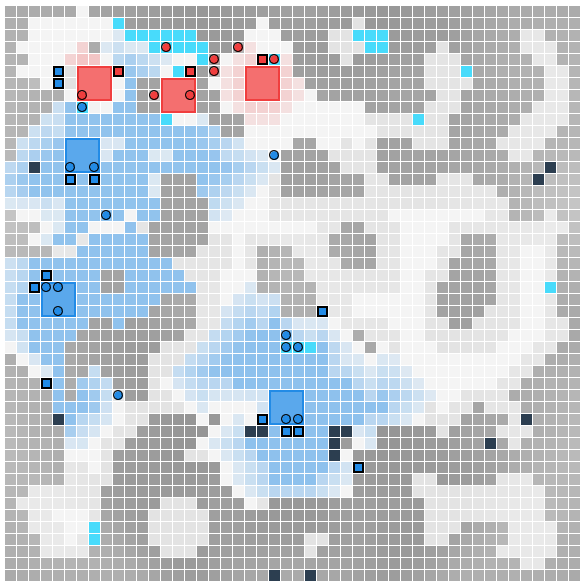
\includegraphics[width=0.4\textwidth]{figures/map.png}
  \caption{%
    An example game board state.
    The resources are \textcolor{ice}{ice}, \textcolor{ore}{ore},
    and rubble is shaded depending on whether it is
    \textcolor{rubblelight!85!black}{light} or \textcolor{rubbledark}{heavy}.
    \textcolor{factory1}{Factories} are the \( 3 \times 3 \) squares with
    \textcolor{factory1}{lichen} growing from them, and robots are the \( 1
    \times 1 \) \textcolor{robot1}{squares} and \textcolor{robot1}{circles}
    (same for the \textcolor{factory2}{other} player).
  }
  \label{fig:map}
\end{figure}

%-------------------------------------------------------------------------
%------------------------------------------------------------------------
\section{Approach}

A single match between two teams is separated into three
phases: the bidding phase, the setup phase, and the main phase.
In the bidding phase, each team bids a certain amount of
resources in order to decide the turn order for the setup phase.
For the sake of simplicity, we choose to ignore the
bidding phase, and simply bid 0 resources every game.
In \autoref{subsec:approach_setup}, we discuss a modeling methodology
for the setup phase based on Gaussian Process regression.
In \autoref{subsec:bandit}, we discuss a black-box hyperparameter
tuning strategy that needs only games between agents.
For the main phase of the game, we utilize an approach inspired by image
segmentation, which we describe in \autoref{subsec:approach_main}.

\subsection{Kernel methods for setup phase}
\label{subsec:approach_setup}

During the setup phase, players take turns selecting a \( 3 \times 3 \) area
which fits within the limits of the board, that does not directly overlap
ice or ore, and is at least 6 tiles from the center of any other factory.
At a high level, our goal during the setup phase is to pick
the ``best'' factory locations that are close to desired
resources, away from the opponent's factories, and so on.

Compared to the main phase of the game, which involves trajectories
of up to 1000 states and actions, each replay only provides around
3-5 data points relevant to the setup phase.
Out of 200,000 total states, we extracted only 203 starting states.
Thus, it is prohibitively expensive to collect a large
amount of data for the setup phase and so we considered
neural networks infeasible at this level of data scarcity.

Instead, we decided to use a kernel method akin to \emph{Gaussian processes}
(GPs), a nonparametric model which directly induces a probability distribution
over functional spaces through its \emph{mean} and \emph{kernel} function, in
order to predict the score of each cell and place a factory at the highest
scoring cells.
Prior information and inductive biases like smoothness
can be injected directly into the kernel information.
As a result, GPs have seen widespread usage in machine learning
\cite{rasmussen2006gaussian} and can be also be seen as the limit of
infinite-depth Bayesian neural networks \cite{bishop2006pattern}.

Specifically, we say a function \( f(\vec{x}) \) is a Gaussian process with
mean function \( \mean(\vec{x}) \) and kernel function \( \K(\vec{x}, \vec{x}')
\) if for any set of points \( X = \{ \vec{x}_i \}_{i = 1}^N \), \( f(X) \sim
\N(\vec{\mean}, \CM) \), where \( \mean_i = \mu(\vec{x}_i) \) and \( \CM_{i,
j} = \K(\vec{x}_i, \vec{x}_j) \).
Given features \( X_\Train = [\vec{x}_1, \dotsc, \vec{x}_N]^{\top}
\) with targets \( \vec{y}_\Train = [y_1, \dotsc, y_N]^{\top} \), we
wish to predict the values at new points \( X_\Pred \) for which \(
\vec{y}_\Pred \) is unknown.
To make predictions at \( X_\Pred \), we condition the desired
prediction \( \vec{y}_\Pred \) on the known data \( \vec{y}_\Train \).
For Gaussian processes, the closed-form posterior distribution is
\begin{align}
  \label{eq:cond_mean}
  \E[\vec{y}_\Pred \mid \vec{y}_\Train] &=
    \vec{\mean}_\Pred +
    \CM_{\Pred, \Train} \CM_{\Train, \Train}^{-1}
    (\vec{y}_\Train - \vec{\mean}_\Train), \\
  \label{eq:cond_cov}
  \Cov[\vec{y}_\Pred \mid \vec{y}_\Train] &=
    \CM_{\Pred, \Pred} -
    \CM_{\Pred, \Train} \CM_{\Train, \Train}^{-1}
    \CM_{\Train, \Pred}.
\end{align}

However, computing the conditional mean \eqref{eq:cond_mean} requires inversion
of the covariance matrix of the training data, which scales as \( \BigO(n^3)
\) for \( n \) training points. In principle we could accelerate this with
state-of-the-art numerics \cite{schafer2021sparse}, but for simplicity we
propose the following approximation: first, without loss of generality we can
assume the mean is \( \vec{0} \) since a nonzero mean will shift every cell
equally, preserving the relative rankings. Second we propose approximating \(
\CM_{\Train, \Train}^{-1} \approx \Id \) which is equivalent to assuming
training cells are statistically independent. We can intuitively
interpret
\begin{align}
  \label{eq:simp_mean}
  \E[\vec{y}_\Pred \mid \vec{y}_\Train] &\approx
    \CM_{\Pred, \Train} \vec{y}_\Train
\end{align}
as a weighted linear combination of training labels, with weights
given by the similarity of each training point to the target point.
We use a separate Mat{\'e}rn kernel for each salient
feature of the board (ice, ore, and rubble) for
\begin{align}
  \label{eq:kernel_pred}
  \vec{y}_\Pred^{\text{final}} &=
    c_{\text{ice}} \vec{y}_\Pred^{\text{ice}}
    + c_{\text{ore}} \vec{y}_\Pred^{\text{ore}}
    + c_{\text{rubble}} \vec{y}_\Pred^{\text{rubble}}.
\end{align}

Other than the coefficient in \eqref{eq:kernel_pred},
each Mat{\'e}rn kernel has two hyperparameters, a length scale which controls
to what degree father points influences the prediction,  and a smoothness
which controls the regularity of sampled functions. We therefore have 12
hyperparameters to learn.

We implement both the estimator and the hyperparameter tuning in the
\texttt{scikit-learn} \cite{pedregosa2011scikitlearn} framework.
We use random search with uniform priors over all coefficients:
\begin{itemize}
  \item Coefficients: \( [-1, 1] \)
  \item Length scale: \( [0, 20] \)
  \item Smoothness: \( \{ 1/2, 3/2, 5/2, \infty \} \)
\end{itemize}

\begin{figure}[t]
  \centering
  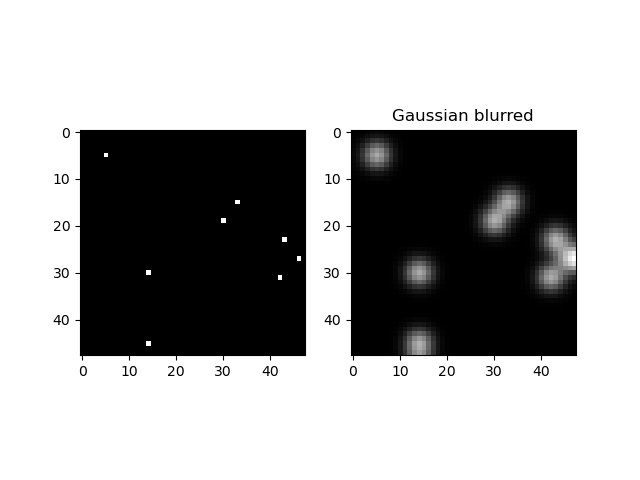
\includegraphics[
    width=0.4\textwidth,
    trim={25px 70px 25px 75px},
    clip,
  ]{figures/factory.png}
  \caption{%
    True factory positions (left) after smoothing (right).
  }
  \label{fig:factory}
\end{figure}

Since we do not have trainable parameters, we do not perform cross
validation and simply take the highest scoring set of parameters.
We score parameters by their mean squared error (MSE) from
\eqref{eq:kernel_pred} to the one-hot encoded true factory positions.
We use Gaussian smoothing to regularize the objective,
encouraging the model to place factories at \emph{similar}
locations to the ground truth (\autoref{fig:factory}).

\begin{table}[h!]
  \begin{center}
  \begin{tabular}{|l|l|}
    \hline
    [coefficients, length scales, smoothness] & MSE \\
    {
      \footnotesize
      [0.061, 0.857, -0.001], [4.21, 1.91, 13.5], [0.5, 0.5, 1.5]
    } & 0.024  \\
    {
      \footnotesize
      [-0.016, 0.460, -0.063], [9.15, 2.75, 0.218], [inf, inf, 0.5]
    } & 0.054 \\
    {
      \footnotesize
      [0.648, 0.434, -0.170], [5.56, 2.33, 0.548], [2.5, 2.5, 0.5]
    } & 0.069 \\
    {
      \footnotesize
      [0.660, 0.270, -0.319], [3.83, 11.3, 0.541], [0.5, 0.5, 0.5]
    } & 0.108 \\
    \hline
  \end{tabular}
  \end{center}
  \caption{%
      Best hyperparameters out of 500 samples for 4 different seeds.
      For each parameter group, the order is [ice, ore, rubble].
  }
  \label{tab:tuning}
\end{table}

The best parameters out of 500 samples for 4
different seeds are shown in \autoref{tab:tuning}.
The model generally encourages placement near ice
and ore while discouraging proximity to rubble.
Through the length scale the model considers distant
ice, nearby ore, but only extremely close rubble.
However, significant variation in the absolute magnitude of
parameters as well as in smoothness suggests the problem
is severely underspecified, probably due to data scarcity.

In addition, we believe that the model may be underscoring valuable
resources like ice and ore due to its inability to encode nearby factories.
In the course of an ordinary game, the first player might place their
factory near ice and ore, thus blocking them from the second player.
Thus factories are artificially far from each other.
In future work we may want to collect data at a more fine-grain level or
model existing factories as electric charges and add an energy penalty.

\subsection{Data and model architecture}
\label{subsec:approach_main}

For the main phase of the game, we utilize a behavioral cloning\cite{cloning}
approach. Specifically, our goal is to predict the actions taken
by each robot that a top-ranking submission would likely perform.
As such, we use the Kaggle API to download replays of games
involving submissions from the top 100 ranked competitors on the leaderboard.
The replay data contains the actions taken by
each robot across all time steps in the game.
We thought that this would lead to a successful strategy
since we would be imitating the already successful,
though unpublished, strategies based on their replays.
% (10 points) What did you do exactly? How did you solve the problem? Why
% did you think it would be successful? Is anything new in your approach?
To achieve this, note that during the main phase of the game, each robot
on the board takes actions as determined by the overall agent/player.
As such, our model's objective can be formulated as to correctly
predict the actions taken by the robots for the replays in our dataset.

% What representations of input and output did the neural
% network expect? How was the data pre/post-processed?
Our model needs to predict the appropriate
action taken by each robot on the board.
Specifically, this involves predicting the type of action (e.g.\ a move to
an adjacent position, a transfer of resources from one robot to another, a
pickup of resources from a factory, etc.), the type of resource for which
the action is being performed, and the quantity of the resource involved
(for transfer/pickup actions).
The treat the prediction of action and resource types as classification
tasks, whereas resource quantity is treated as a regression problem.

% What was the structure of your problem? How did the structure
% of your model reflect the structure of your problem?
As such, the structure of our problem is that we are given a
representation of the current board state, which includes
the locations of the factories, resources, and robots.
Clearly, this leads to a 2D-grid structure spread across multiple channels.
Likewise, the output is to predict the values described above for
certain positions in the board, also resulting in a 2D-grid structure.
This problem can naturally be interpreted as a form of
image segmentation, which is generally the idea of predicting
from a discrete class of values for each pixel in an image.

Thus, we design our model in a similar method to image segmentation,
except with the modification that we have three output heads mentioned
above, and not just a pixel-wise single classification objective.
Additionally, rather than a 3-channel input like with images, our input
contains 37 channels due needing to account for all items on the board.

Therefore, we structure our model with an image segmentation
backbone architecture, such as U-Nets \cite{u-net} and LRASPP
\cite{lraspp}, followed by three fully-connected portions for
the output heads at each position in the board.
For the backbone, we consider using a simple linear model as a baseline, which
is implemented via a single convolutional layer with a kernel size of 1.
We also consider U-Net, which is an improvement over encoder-decoder fully
connected convolutional networks for segmentation due to the presence
of skip connections and multiple up-sampling layers rather than only 1.
Lastly, we consider LRASPP, which is a lightweight image
segmentation model designed to be run on mobile devices.
We do so since we are not using the pretrained version of any models
(as it does not make sense to use models trained on actual images for
a problem that is not involving images) in this problem, and thus the
larger U-Net may not be able to learn efficiently on our dataset.

% What parts of your model had learned parameters (e.g.,
% convolution layers) and what parts did not (e.g.,
% post-processing classifier probabilities into decisions)?
In total, all components related to the
segmentation and output heads are learnable.
The only non-learnable parameters of this model include
our pre-processing to convert the raw replays into PyTorch tensors for the
model to take as input and output (for training), as well as the logic for
converting the model's output into decisions to make in-game, which can be
done by using the argmax for the classification outputs and rounding to the
nearest integer for the regression output.

% (5 points) What problems did you anticipate? What problems
% did you encounter? Did the very first thing you tried work?
The main problem that we anticipated with approach was
feature scaling for real-valued inputs in the board,
such as the number of a given resource on a position.
Since these values could potentially get large and thus hinder the
model's accuracy, we instead used the log of all real-valued features,
a trick which has been used in other settings \cite{scaling}.
Additionally, we anticipated an issue with balancing our loss
function to accurately account for all 3 output heads, which
we addressed by weighing the loss in \autoref{sec:training}.
Lastly, there was a class imbalance as certain actions were
taken much more frequently than others in our replays.
We attempted to address this using the recall-based class
weighting approach suggested in~\cite{imbalance}, but found that
this approach did not have a significant impact on performance.

\begin{figure*}
  \centering
  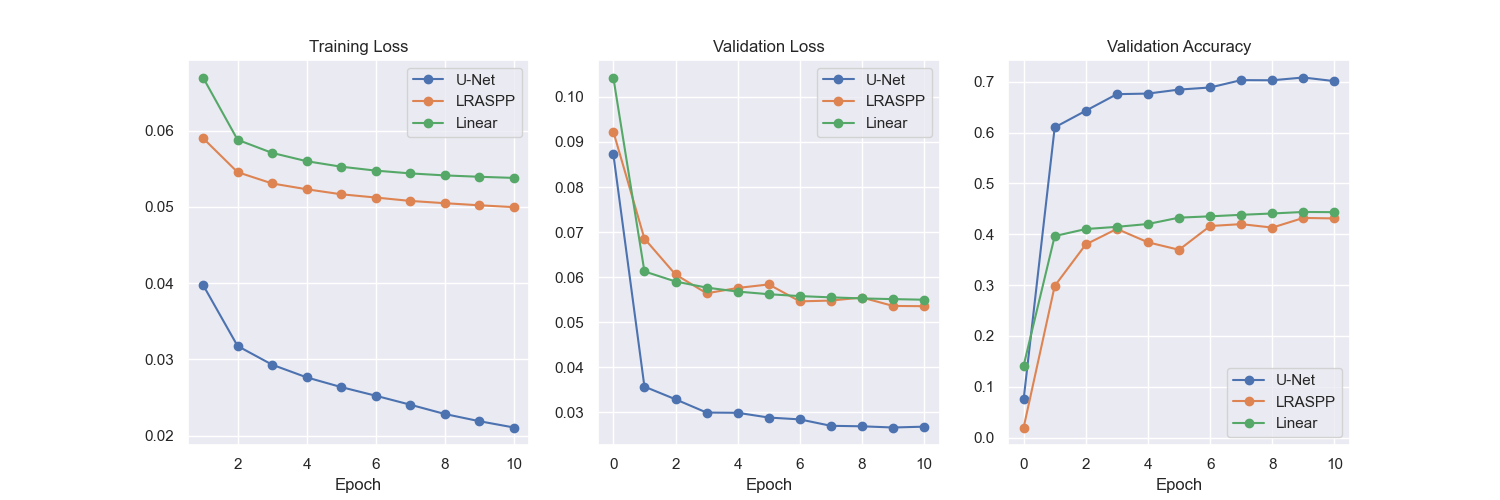
\includegraphics[width=\textwidth]{figures/results.png}
  \caption{
    The training loss, validation loss, and validation
    accuracy of our model for each of the three architectures.
  }
  \label{fig:results}
\end{figure*}

\begin{figure*}
  \centering
  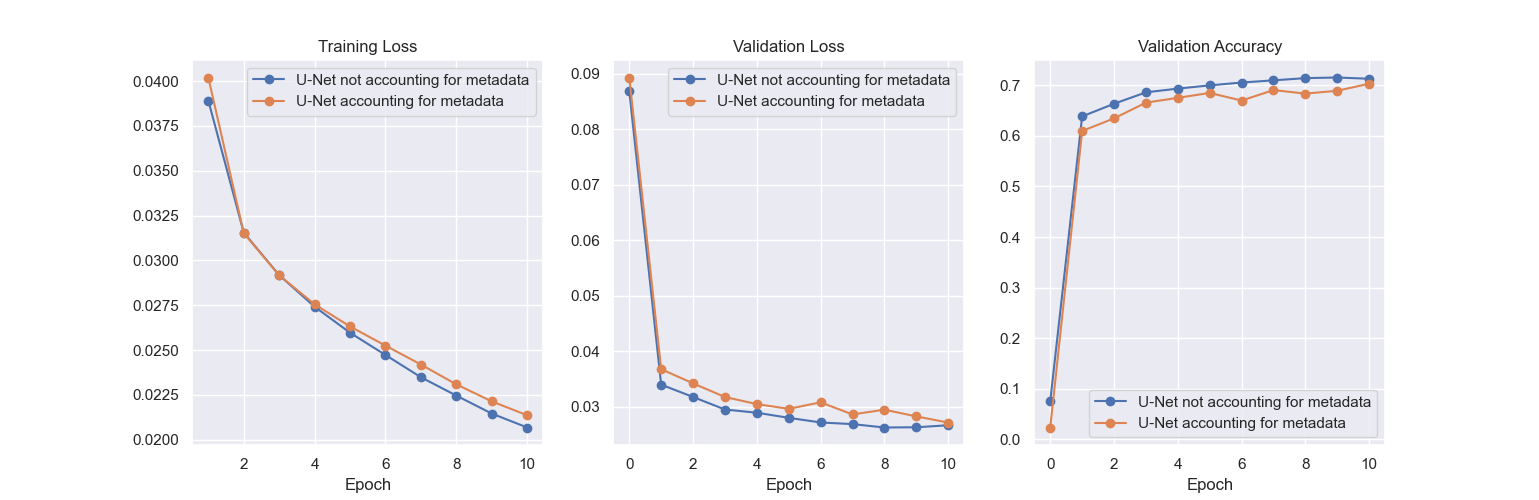
\includegraphics[width=\textwidth]{figures/unet_meta.png}
  \caption{%
    Curves for training loss, validation loss, and validation
    accuracy of our approach with the U-Net architecture,
    comparing performance with and without metadata.
  }
  \label{fig:u_net}
\end{figure*}

\section{Training}
\label{sec:training}

For training our model on the main phase of the game, we use the same
loss function regardless of the underlying segmentation architecture.
Specifically, since our model needs to predict the type of action, resource
involved, and quantity at each position, our loss function can be written as
\begin{align}
  \label{eq:train_loss}
  L &=
    L_{\text{action type}}
    + L_{\text{resource}}
    + \alpha L_{\text{quantity}}.
\end{align}

Prediction of action type and resource are both classification problems, so
we perform pixel-wise cross-entropy loss for both, taking the mean across the
entire board and applying a 0/1 mask, so that the loss only includes positions
at which there is a robot.
For predicting the quantity, we have a regression problem,
so we use pixel-wise mean squared error, taking the sum
across the entire board and applying a 0/1 mask again.
$\alpha$ is a non-negative hyperparameter used to weigh the MSE
loss, in order to prevent it from dominating the cross-entropy loss.

% What hyperparameters did the model have? How were they chosen?
% How did they affect performance? What optimizer was used?
The hyperparameters of our model mainly include the learning
rate, MSE weight term, and the coefficient of weight decay.
We tune hyperparameters via a coarse grid search up to 1 step per decade.
We trained using the Adam optimizer with a minibatch size of 16 for 10 epochs.
We ended up using a learning rate of a learning rate of
1e-3, weight decay of 1e-6, and $\alpha=1/100$, which we
found performed relatively well on all architectures.

We used \texttt{PyTorch} \cite{paszke2019pytorch} for our model implementation,
and obtained implementations of the baseline semantic segmentation
architectures from \texttt{Torchvision} \cite{maintainers2016torchvision}.
We did not use pretrained weights in any form, as our domain does
not deal with a visual image-based input in the traditional sense.

\subsection{Conditioning on Demonstrator Quality}
\label{sec:metadata}

We consider passing in various types of metadata available
in the replay files, in addition to the board state itself.
This includes information
about the two players' ratings, as well as the difference in final
score (the accumulated lichen), which determines the game winner.
We add these scalars to the input by broadcasting over the entire
input plane and appending them as additional image channels.
This approach was loosely inspired by the Return-To-Go (RtG) input provided
during the training of Decision Transformers \cite{decision_transformers}.
Essentially, by treating the problem as a sequence modeling task and
conditioning on the reward received in the remainder of the episode, the
decision transformer learns to model both effective and ineffective actions.
By including data about player ratings and the future match outcome into
our training data, and conditioning on \emph{high} player ratings or
\emph{winning} match outcomes at test time, we hope to attain similar benefits.

\paragraph{Remark}

We initially planned on using a reinforcement learning approach for
this problem rather than the presented supervised learning model,
and in \autoref{subsec:bandit}, we experimented with a more rigorous
dueling bandit approach to hyperparameter tuning.
However, we shifted away from reinforcement learning due to challenges with
the LuxAI environment, and thus for this supervised learning problem, simply
evaluating hyperparameters on a validation set is a more scalable approach
with our magnitude of training data.

\section{Experiments and Results}
\label{sec:results}

Our primary measure of success was to consider the accuracy of our
model on the validation dataset in predicting the action type,
resource, and quantity (see above) for each robot on the board.
We considered this metric under the various semantic
segmentation architectures mentioned earlier.
The training and accuracy curves can be seen in \autoref{fig:results}.
It should be worth noting that we are not using the pretrained version
of these models since they are pretrained for images; although this task
involves a pointwise prediction on grid-like structures, they are not images.
As such, we consider all such architectures rather than relying
on whichever performs best on benchmark image datasets.
Based on the figure, the U-Net architecture has the
strongest performance, while the performance of LRASPP is
somewhat similar or slightly worse than the linear model.

% Did the model overfit? How well did the approach generalize?

\subsection{Ablation: metadata conditioning}\label{sec:results:metadata}

We conduct an ablation study of the additional metadata input channels
described in \autoref{sec:metadata} by comparing performance including the
metadata and performance without (where the initial channels are set to zero).
To isolate the impact of this change, we test
with the only best-performing U-Net architecture.

The training curves comparing the two
approaches are depicted in \autoref{fig:u_net}.
There does not seem to be a significant difference
in performance with and without the metadata.
We discuss possible interpretations and alternative
approaches in \autoref{sec:discussion}.

% \textbf{
%   Important: This section should be rigorous and thorough. Present
%   detailed information about decision you made, why you made them, and
%   any evidence/experimentation to back them up. This is especially
%   true if you leveraged existing architectures, pre-trained models,
%   and code (i.e. do not just show results of fine-tuning a pre-trained
%   model without any analysis, claims/evidence, and conclusions, as
%   that tends to not make a strong project).
% }

\section{Discussion}
\label{sec:discussion}

Of the 3 semantic segmentation architectures tested with our model for the
main phase, the U-Net performed the best. The poor performance of the baseline
linear model is unsurprising, due to the limited model capacity. However,
LRASPP surprisingly performed quite poorly, even relative to the linear
approach. One possible explanation is that during inference, the LRASPP
architecture predicts at a lower resolution before bilinearly interpolating
the output to a higher resolution. Although this may be a reasonable
architectural decision for typical tasks involving semantic segmentation of
images (after all, adjacent pixels likely belong to the same object class),
in this problem space it is quite common for robots in adjacent tiles to
take entirely distinct actions, thus reducing LRASPP's effectiveness.

In \autoref{sec:results:metadata} we observed that conditioning on submission
ratings and match outcomes did not improve training or validation performance.
This outcome is not entirely unexpected, as we do not take the
sequence modeling approach from~\cite{decision_transformers}, so
similar modeling decisions may not lead to strong improvements
in the domain of single-step modeling.
In addition, our source of data was replays from the top 100 agents, during
a snapshot of the leaderboard relatively early on in the competition.
At that point, most of the agents were likely deterministic, heuristic-based
agents, whose behavior did not change much regardless of how well the team was
doing at a particular phase of the game, and was of course fixed regardless of
the submission's current rating.

\subsection{Analysis: post-competition comparison to other approaches}
\label{sec:discussion:compare}

By combining the kernel methods for the setup phase with the
segmentation approaches for the main phase of the game, we technically
have an agent capable of competing in the Lux AI environment.
However, despite the high overall accuracy on the offline dataset,
we ran into several difficulties when deploying the model online.
For example, the agent would often fail to mine
sufficient quantities of ice to survive past turn 150.

After the competition ended on April 24th, we can compare our
approach with various solutions other teams decided to publish.
We noticed that the imitation-based solution posted
\href{https://www.kaggle.com/competitions/lux-ai-season-2/discussion/404842}{%
  here%
} for example, was quite similar to our work.
Notable difference from our method include
\begin{itemize}
    \item A simplification of the action space: they only
      predicted action classes, and used hardcoded parameters
      for those actions (target resource and quantity).
    \item No demonstration heterogeneity: all of their replays
      came from a single, reinforcement-learning based submission,
      while we sampled uniformly from the top 100 players.
    \item More sophisticated postprocessing: they masked out
      invalid actions, as well as friendly inter-robot collisions.
    \item Heuristic algorithm for the setup phase, based on human intuition.
\end{itemize}
Essentially, for the main phase of the game, their
approach puts strict limitations on the output space
of the model, reducing the difficulty of the problem.
A lack of demonstration heterogeneity may lead to
reduced strategic diversity, but also meant that their
targets would be more consistent across their dataset.

\section{Conclusion}

In this project, we explored a deep imitation
learning approach to the LuxAI Season 2 competition.
Specifically, we used a kernel method approach for the setup
phase and an image segmentation approach to the main phase.
We experimented with multiple segmentation architectures
and found that U-Nets worked best for this task.
Furthermore, we also considered usage of the game's metadata
values in our model to see if there would be further improvement.

%-------------------------------------------------------------------------

\clearpage

{
  \small
  \bibliographystyle{ieee_fullname}
  \bibliography{egbib}
}

\begin{table*}[t]
  \begin{center}
  \begin{tabular}{|l|c|l|}
    \hline
    Student Name & Contributed Aspects & Details \\
    \hline\hline
    Stephen Huan
      & Setup phase, hyperparameter tuning, report writing
      & Kernel methods, dueling bandit algorithms \\
    Daniel Lu
      & Training, experimentation, report writing
      & Tuning framework, architecture, initial classifier \\
    Vedaant Shah
      & Training, architecture, report writing
      & Overall training and U-Net implementations \\
    Jerry Xiong
      & Dataset, preprocessing, report writing
      & Created the dataset and preprocessing pipeline \\
    \hline
  \end{tabular}
  \end{center}
  \caption{Contributions of team members.}
  \label{tab:contributions}
\end{table*}

\appendix

\section{Source code}

Code for all experiments can be found at the repository
{%
  \url{https://github.com/jxiong21029/LuxS2}%
}.

\section{Work division}

% Please add a section on the delegation of work among team members at the
% end of the report, in the form of a table and paragraph description.
% This and references do \textbf{NOT} count towards your page limit.
% An example has been provided in Table \ref{tab:contributions}.

The contributions of each team member is as follows.
See also \autoref{tab:contributions} for a high-level summary.

\paragraph{Stephen Huan}

I primarily worked on analyzing factory placement in the setup
phase and developing a possible hyperparameter tuning strategy.
For the setup phase I decided to use a kernel method
inspired by Gaussian processes, and coded the estimator,
hyperparameter tuning, and integration into the final agent.
I also worked on developing the hyperparameter tuning algorithm
with dueling bandits, implementing four different papers.
Correspondingly, I wrote \autoref{subsec:approach_setup}
and \autoref{subsec:bandit} of this report.

\paragraph{Daniel Lu}

I worked on training and hyperparameter tuning. This involved
integrating our chosen models, dataset, and parameter
specification into a custom tuning framework, as well as
performing the training and creating visualizations.
Additionally, I worked on a classifier for an early iteration
of the setup phase inspired by Monte-Carlo Tree Search and
contributed towards applying the chosen architectures.
In the report, I focused on the introductory \autoref{sec:intro}
(\autoref{subsec:problem} and \autoref{subsec:motivation}).

\paragraph{Vedaant Shah}

I worked on creating the logic for training and
evaluating our model for the main phase of the game.
This included writing the loss function, the training
loop over the dataset, and the evaluation function
I also implemented the U-Net architecture in our code
as well as the logic for the model using the metadata.
I trained and obtained the results for the model with the
U-Net architecture both with and without the metadata.
As such, I wrote significant portions of \autoref{subsec:approach_main},
\autoref{sec:training}, and \autoref{sec:results}.

\paragraph{Jerry Xiong}

In the early phases of the project, I explored a deep
reinforcement learning based approach for this environment.
The bandit-based hyperparameter tuning approach I encouraged
Stephen to work on was an offshoot of this effort.
However, we eventually decided that this was outside the
scope of what we could accomplish in this timeframe.
After pivoting to an imitation learning approach, my main contributions were
downloading and processing the dataset into a format consumable by neural
networks, including the board state and metadata inputs and the action targets.
I also experimented with the recall-based action class-weighting approach.
I contributed to \autoref{sec:intro}, \autoref{sec:metadata},
\autoref{sec:results:metadata}, and \autoref{sec:discussion} of the report.

\clearpage

\section{Dueling bandits for hyperparameter tuning}
\label{subsec:bandit}

Initially, we implemented a reinforcement learning approach for the main
phase of the game with an agent playing and learning from its actions.
Due to challenges with the Lux AI environment, we
switched to the segmentation-based supervised learning
approach discussed in \autoref{subsec:approach_main}.
In this setting, different agents can be compared by their supervised loss.
Here we present our initial ideas of comparing
agents with only black-box game evaluations.

Given two agents, the most natural way to
compare them is to play them against each other.
However, because of the inherent stochasticity in the game and
agent strategies, this is a relatively noisy comparison, perhaps
requiring multiple comparisons to determine which is better.
We consider determining the best agent from \( K \) agents
in the least number of comparisons, as each comparison
requires an computationally expensive simulation of the game.
These \( K \) agents will eventually be models with different hyperparameters.

We model this in the \emph{multi-armed dueling bandit} framework.
While we could use existing probably approximately correct (PAC) algorithms
for maxing and ranking \cite{falahatgar2017maxing}, often they make stringent
assumptions on the problem structure like strong stochastic transitivity (SST).
Instead, we will seek nearly assumptionless algorithms.
Since we can run multiple games in parallel, the \emph{batched} algorithms
of \cite{agarwal2022batched, agarwal2022asymptotically} are compelling, but
we believe the overhead of adapting a sequential algorithm to the parallel
setting is not significant.

Following the setup of \cite{wu2016double}, consider \( K \) arms.
For the \( t \)-th timestep the algorithm selects two arms \( (a_t^{(1)},
a_t^{(2)}) \) and receives win (1) or loss (0) based on some preference
matrix \( p \) such that \( \Prob \{ i \succ j \} \defeq p_{i, j} \) where
\( i \succ j \) means that \( i \) won.
We assume \( p_{i, j} + p_{j, i} = 1 \) and \( p_{i, i} \defeq 1/2 \) and
we say an arm \( i \) \emph{beats} arm \( j \) if \( p_{i, j} > 1/2 \).

There are many notions of a ``best'' arm, here we consider two.
A \emph{Condorcet} winner is an arm that beats all other
arms, and may not exist for every preference matrix.
A natural relaxation that always exists is a \emph{Copeland} winner,
which is the arm(s) that beats the most number of other arms.
Note that a Condorcet winner (when it exists) is
always a Copeland winner but the converse is not true.

Specifically, define the (normalized) Copeland score to be
\( \zeta_i \defeq \frac{1}{K - 1} \sum_{j \neq i} \Ind(p_{i, j} > 1/2)
\) where \( \Ind(\cdot) \) is the indicator function.
Let \( \zeta^* \defeq \max_{1 \leq i \leq K} \zeta_i \) be the
maximum score; an arm \( i \) is a Copeland winner if \( \zeta_i
= \zeta^* \) and a Condorcet winner if \( \zeta_i = 1 \).
We define the expected cumulative \emph{Copeland
regret} of a dueling bandit algorithm to be
\begin{align}
  \label{eq:regret_copeland}
  R(T) \defeq
    \zeta^* T - \frac{1}{2} \sum_{t = 1}^T \E \left [
      \zeta_{a_t^{(1)}} + \zeta_{a_t^{(2)}}
    \right ]
\end{align}
or intuitively, the accumulated difference
from the optimal arm over \( T \) timesteps.
Since the regret \eqref{eq:regret_copeland} penalizes unnecessary
comparisons, it can be applied to many notions of regret.
We also define the similar \emph{Condorcet regret} \cite{saha2022versatile}
where the arm \( a^{(\cw)} \) is the Condorcet winner as
\begin{align}
  \label{eq:regret_condorcet}
  R^{\cw}(T) \defeq
    \frac{1}{2} \sum_{t = 1}^T \left [
      \Delta(a^{(\cw)}, a_t^{(1)})
      + \Delta(a^{(\cw)}, a_t^{(2)})
    \right ]
\end{align}
where \( \Delta(i, j) \defeq p_{i, j} - 1/2 \) is
the optimality gap between arm \( i \) and \( j \).
We now give an overview of existing methods:
\begin{itemize}
  \item Beat the mean (BTM) \cite{yue2011beat}
  \item Scalable Copeland bandits (SCB) \cite{zoghi2015copeland}
  \item Relative minimum empirical divergence (RMED) \cite{komiyama2015regret}
  \item Copeland winners RMED (CW-RMED) \cite{komiyama2016copeland}
  \item Double Thompson sampling (DTS) \cite{wu2016double}
  \item Versatile dueling bandits (VDB) \cite{saha2022versatile}
\end{itemize}

BTM assumes a total ordering, i.e.\ \( a_1 \succ \dotsb \succ a_K \), a
(relaxed) stochastic transitivity in the sense that for some \( \gamma
\geq 1 \) and triplet of arms \( a_i \succ a_j \succ a_k \), it holds \(
\gamma \Delta(i, k) \geq \max \{ \Delta(i, j), \Delta(j, k) \} \), and
a stochastic triangle inequality in the sense that \( \Delta(i, k) \leq
\Delta(i, j) + \Delta(j, k) \).
It has regret \( \mathcal{O}(\frac{\gamma^7 K}{\Delta^*} \log T) \) where \(
\Delta^* \defeq \min_{i \neq a^{(\cw)}} \Delta(a^{(\cw)}, i) \) which can be
adapted to find a \( (\varepsilon, \delta) \)-PAC optimal bandit \( \hat{a}
\) in the sense that \( \Prob\{ \Delta(a^{(\cw)}, \hat{a}) > \varepsilon
\} \leq \delta \) with sample complexity \( \mathcal{O}(\frac{\gamma^6
K}{\varepsilon^2} \log \frac{K N}{\delta} ) \) for \( N \defeq \ceil{\frac{36
\gamma^6}{\varepsilon^2} \log \frac{K^3 N}{\delta}} \).

With probability \( 1 - \delta \) SCB finds a \( \varepsilon \)-Copeland
winner \( \hat{a} \) in the sense that \( 1 - \zeta_{\hat{a}} \leq (1 -
\zeta^*)(1 + \varepsilon) \) with accumulated total regret of the form \(
\mathcal{O}(K \log K \log T) \).

RMED finds a Condorcet winner with (asymptotically optimal) regret \(
\mathcal{O}(\sum_{i \neq a^{(\cw)}} \frac{\log T}{\Delta(a^{(\cw)},
i)}) \) but includes an undesirable \( \mathcal{O}(K^2) \) dependency.
CW-RMED is an extension of RMED to the
Copeland winner with similar performance.

DTS uses Thompson sampling twice to select both arms.
DTS+ is a slight improvement which cleverly breaks ties.
DTS achieves a Copeland regret of \( \mathcal{O}(K^2 \log T) \) but
this analysis is probably not tight as it performs well in practice.

VDB uses a simple reduction from dueling bandits
to independent standard multi-armed bandits.
It uses the ``best-of-both-world'' algorithm Tsallis-INF
\cite{zimmert2022tsallisinf} that achieves both the optimal (pseudo-)regret
\(
\mathcal{O}(\sum_{i \neq a^{(\cw)}} \frac{\log T}{\Delta(a^{(\cw)}, i)})
\) in the stochastic case and \( \mathcal{O}(\sqrt{KT}) \) regret in the
adversarial case where at every timestep the preference matrix \( p_{i,
j} \) is allowed to change in response to the bandit algorithm.
VDB basically inherits these regret bounds but its analysis
depends significantly on the existence of a Condorcet winner.

We consider four variants of VDB depending on whether reduced-variance (RV)
estimators are used for the loss \cite{zimmert2022tsallisinf} and whether the
bandits share information by re-using the same online mirror descent update
(remark 2 of \cite{saha2022versatile}).

\begin{figure}
  \centering
  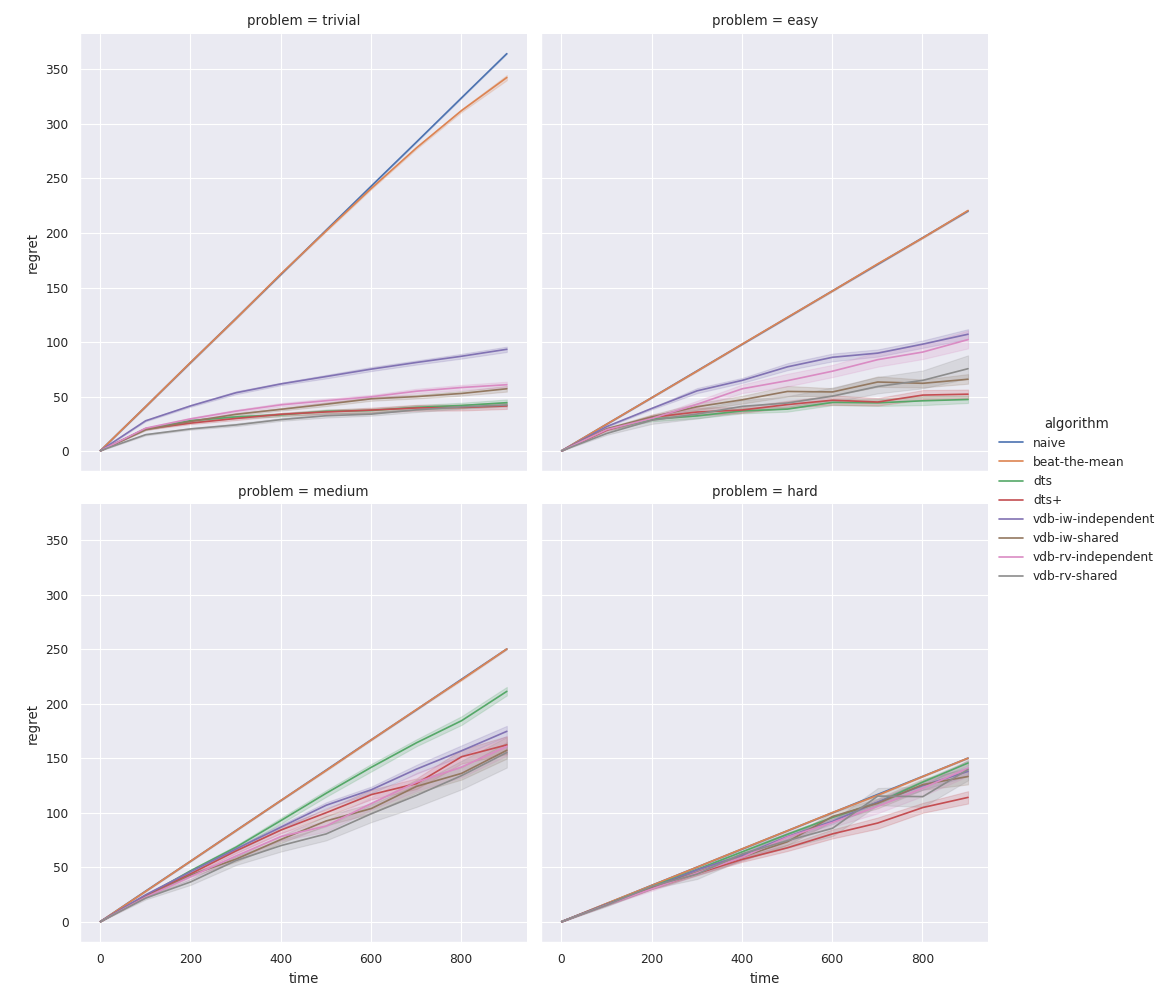
\includegraphics[width=0.45\textwidth]{figures/regret_1.png}
  \caption{%
    Regret for \( T = 1000 \), \( 50 \) trials per timestep.
  }
  \label{fig:regret1}
\end{figure}

We implemented BTM, SCB, DTS and DTS+, and
the four aforementioned variants of VDB.
Results for SCB are not shown due to
difficulties with its experimental results.

We consider four experimental setups, in order of decreasing
structural assumptions on the preference matrix \( p \):
\begin{itemize}
  \item ``trivial'': We use the Bradley–Terry–Luce
    (BTL) or Plackett-Luce model \cite{saha2022versatile}.
    Given a list of real scores \( r_1, \dotsc, r_K \), the probability arm \(
    i \) beats arm \( j \) is defined as \( e^{r_i}/(e^{r_i} + e^{r_j}) \).
    This guarantees a total ordering (and therefore a Condorcet winner),
    stochastic transitivity, and the stochastic triangle inequality.
    We sample \( r_i \) independently and
    identically (i.i.d) from \( \Uniform(0, 100) \).
  \item ``easy'': We generate a preference
    matrix \( p \) with entries taken i.i.d. \( p_{i, j}
    \sim \Uniform(0, 1) \) for \( 2 \leq i < j \leq K \).
    We then take \( p_{1, j} \sim \Uniform(1/2, 1) \) for \( 2 \leq j
    \), guaranteeing that the arm \( i = 1 \) is a Condorcet winner.
  \item ``medium:``: We generate random matrices with entries i.i.d. \(
    p_{i, j} \sim \Uniform(0, 1) \) for \( 1 \leq i < j \leq K \ \) until
    \( p \) has multiple \( (> 1) \) Copeland winners.
  \item ``hard'': We generate a random matrix like medium
    but without resampling for multiple Copeland winners.
\end{itemize}

For all setups we take \( K = 10 \) arms and shuffle the preference
matrix after every trial to remove possible bias from the ordering.
Experiments were implemented using standard Python
scientific libraries \texttt{numpy} \cite{harris2020array}
and \texttt{scipy} \cite{virtanen2020scipy}.
Plots were produced with \texttt{matplotlib} \cite{hunter2007matplotlib}
and \texttt{seaborn} \cite{waskom2021seaborn},
which generated the shaded confidence intervals.

\begin{figure}
  \centering
  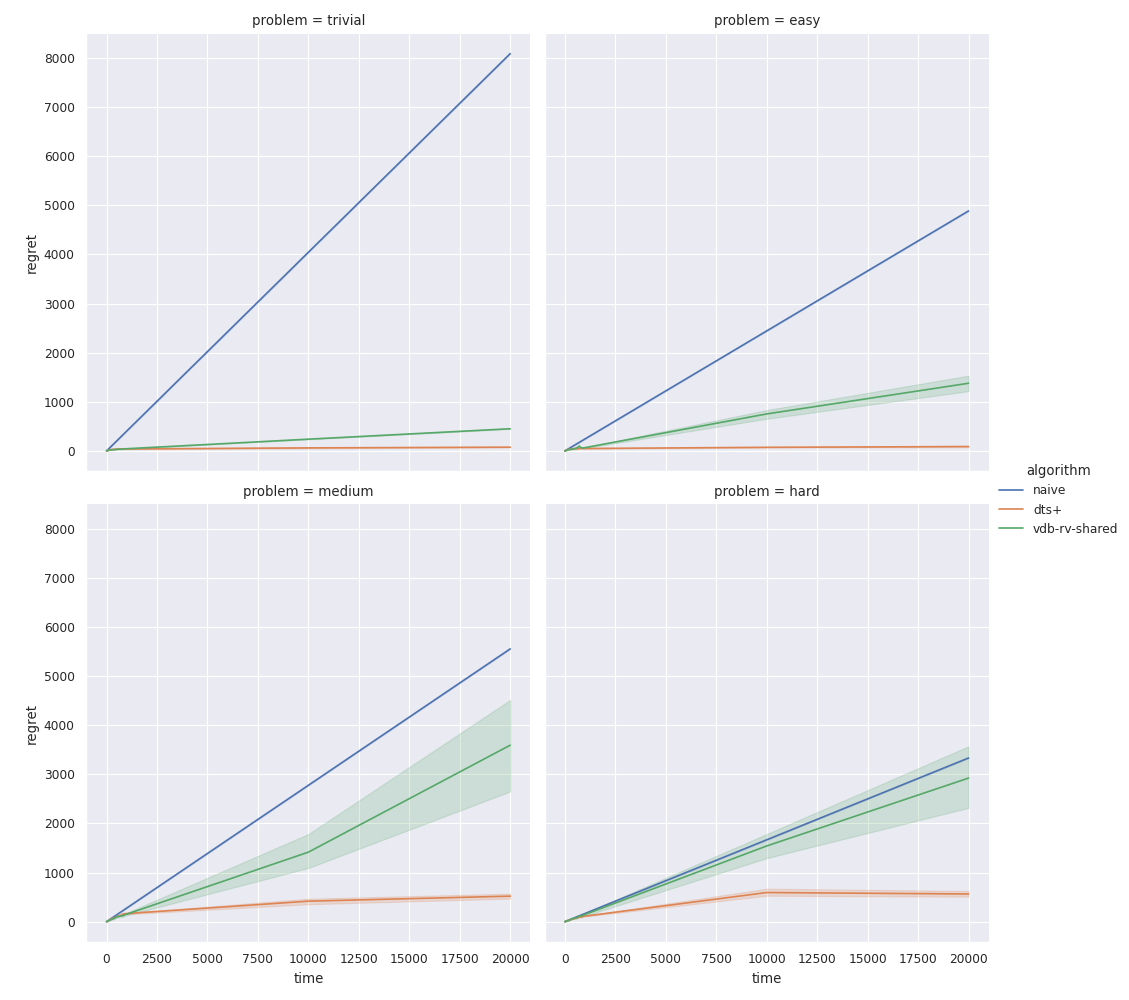
\includegraphics[width=0.43\textwidth]{figures/regret_2.png}
  \caption{%
    Regret for \( T = 20,000 \), \( 10 \) trials per timestep.
  }
  \label{fig:regret2}
\end{figure}

As shown in \autoref{fig:regret1}, DTS+ performs the best or
close to the best over all setups, and of the VDB variants the
reduced-variance estimator with shared information is the best.
BTM is barely better than a naive strategy
which simply samples every pair of arms evenly.
For the more difficult setups, the regret of DTS+ and VDB look linear
despite their theoretical regret of \( \mathcal{O}(\log T) \).
Running for a longer time horizon (\autoref{fig:regret2}) shows that
DTS+ achieves log scaling while VDB's regret still looks linear.

\begin{figure}[h!]
  \centering
  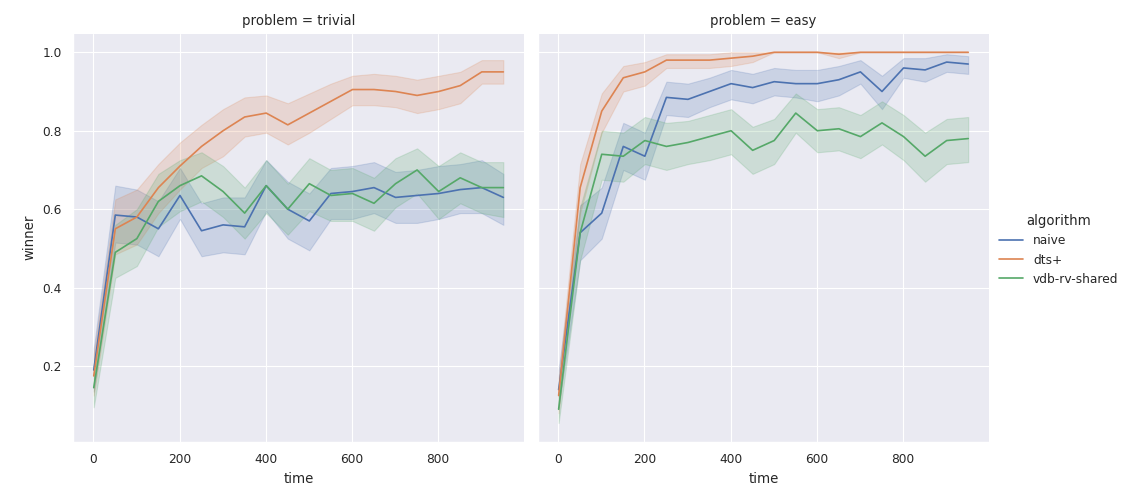
\includegraphics[width=0.44\textwidth]{figures/winner_3.png}
  \caption{%
    Winner recovery rate for \( T = 1000 \), \( 200 \) trials.
  }
  \label{fig:winner3}
\end{figure}

Finally, \autoref{fig:winner3} shows the percentage
chance the algorithm recovers the Condorcet winner.
DTS+ performs significantly better than the naive strategy, while
VDB is about the same or even worse on the harder problem setup.

We think that existing algorithms focus too heavily on
(1) regret minimization and (2) asymptotic scaling.
In our use case, we only want to recover the best arm
and do not mind making poor comparisons along the way.
We also cannot afford taking \( T \to \infty \),
instead, we need good performance for \( T \ll 10^3 \).
Whether an algorithm with these performance
characteristics exists is an open question.

\end{document}
